\documentclass[11pt,a4paper]{article}

% ADDED PACKAGE
\usepackage{latexsym}
\usepackage{amssymb}
\usepackage{amsmath}
\usepackage{graphicx}   %  include figure files
\usepackage{epsfig}       %  files .eps
\usepackage{dcolumn}   %  align tble columns on decimal points
\usepackage{bm}           %  bold math
\usepackage{color}        %  textcolor
\usepackage{ulem}        %  sout (strike out)
%\usepackage{wrapfig}
%tommaso
\usepackage{tabularx}
\usepackage[T1]{fontenc}
\usepackage{hyperref}
\usepackage{times}
\usepackage{floatflt}
\renewcommand{\abstractname}{Summary}

\usepackage[top=50pt,bottom=50pt,left=50pt,right=50pt]{geometry}

\usepackage{listings}
\usepackage{color}

\definecolor{mygreen}{rgb}{0,0.6,0}
\definecolor{mygray}{rgb}{0.5,0.5,0.5}
\definecolor{mymauve}{rgb}{0.58,0,0.82}

\lstset{ %
  basicstyle=\linespread{0.85}\ttfamily\footnotesize,        % the size of the fonts that are used for the code
  breakatwhitespace=false,         % sets if automatic breaks should only happen at whitespace
  breaklines=true,                 % sets automatic line breaking
  captionpos=b,                    % sets the caption-position to bottom
  commentstyle=\color{mygreen},    % comment style
  deletekeywords={...},            % if you want to delete keywords from the given language
  escapeinside={\%*}{*)},          % if you want to add LaTeX within your code
  extendedchars=true,              % lets you use non-ASCII characters; for 8-bits encodings only, does not work with UTF-8
  keepspaces=true,                 % keeps spaces in text, useful for keeping indentation of code (possibly needs columns=flexible)
  keywordstyle=\color{blue},       % keyword style
  language=Python,                 % the language of the code
  otherkeywords={*,...},            % if you want to add more keywords to the set
  numbers=left,                    % where to put the line-numbers; possible values are (none, left, right)
  numbersep=5pt,                   % how far the line-numbers are from the code
  numberstyle=\tiny\color{black}, % the style that is used for the line-numbers
  rulecolor=\color{black},         % if not set, the frame-color may be changed on line-breaks within not-black text (e.g. comments (green here))
  showspaces=false,                % show spaces everywhere adding particular underscores; it overrides 'showstringspaces'
  showstringspaces=false,          % underline spaces within strings only
  showtabs=false,                  % show tabs within strings adding particular underscores
  stepnumber=1,                    % the step between two line-numbers. If it's 1, each line will be numbered
  stringstyle=\color{mymauve},     % string literal style
  tabsize=2,	                   % sets default tabsize to 2 spaces
}

% NEW COMMAND
\newcommand{\vE}{\mathbf{E}}
\newcommand{\vB}{\mathbf{B}}
\newcommand{\vJ}{\mathbf{J}}
\newcommand{\vx}{\mathbf{x}}
\newcommand{\vp}{\mathbf{p}}
\newcommand{\vv}{\mathbf{v}}
\newcommand{\vu}{\mathbf{u}}
\newcommand{\vF}{\mathbf{F}}



\begin{document}
%-------
% Title
%-------
\title{TP - UPMC \\ Introduction to plasma physics with Particle-In-Cell simulations}


\author{Caterina~Riconda \footnote{\url{caterina.riconda@upmc.fr}}, \and Tommaso Vinci \footnote{\url{tommaso.vinci@polytechnique.edu}}, \and Mickael~Grech \footnote{\url{mickael.grech@polytechnique.edu}} }

\date{}

\maketitle              

\vspace*{-20pt}
\hrule
\section*{Summary}
These exercises are intended as an introduction to plasma physics through Particle-in-cell (PIC) simulation.
We first give some details on the open-source PIC code SMILEI (\url{http://www.maisondelasimulation.fr/smilei}) currently developed at LULI in collaboration with various laboratories.

We propose two projects: 
\begin{enumerate}
\item electron plasma waves.
\item two-stream instability.
\end{enumerate}


%\tableofcontents


%%%%%%%%%%%%%%%%%%
%  INTRODUCTION  %
%%%%%%%%%%%%%%%%%%
\section*{Introduction}\label{intro}

\subsection*{The Particle-In-Cell code SMILEI}

SMILEI is a Particle-In-Cell (PIC) code initially developed to study laser-plasma interaction at extreme intensities. 
The PIC method aims at solving the Maxwell-Vlasov system of  equations~\cite{birdsall_langdon}.

The electromagnetic fields ($\vE,\vB$) are described on a (here cartesian) grid, and Maxwell's equations:
\begin{subequations}\label{eq_Maxwell}
\begin{eqnarray}
\nabla \cdot \vE &=& \frac{\rho}{\epsilon_0} \,,\\
\nabla \cdot \vB &=& 0 \,,\\
\nabla \times \vE &=& -\partial_t \vB \,,\\
\nabla \times \vB &=& \mu_0\, \vJ + \mu_0 \epsilon_0\,\partial_t \vE \,,
\end{eqnarray}
\end{subequations}
are solved using the finite-domain time-difference (FDTD) method~\cite{taflove_2005}.
In Eqs.~\eqref{eq_Maxwell}, $\epsilon_0$ and $\mu_0$ are the vacuum permittivity and permeability, respectively. 
As for $\rho$ and $\vJ$, they denote the total charge density and total current, respectively.

Both quantities $\rho$ and $\vJ$ are due to the presence of a plasma.
The kinetic description of a collisionless (fully ionised) plasma is encompassed by the (here relativistic) Vlasov equation, which for each species $s$ of the plasma, reads:
\begin{eqnarray}\label{eq_Vlasov}
\left(\partial_t  + \frac{\vp}{m_s \gamma} \cdot \nabla + \vF_L \cdot \nabla_{\vp} \right) f_s = 0\,,
\end{eqnarray}
where $f_s(t,\vx,\vv)$ is the species distribution function, $\vF_L$ is the external force acting on the species (in our case the Lorentz force), $m_s$ is the mass of one (physical) element of species $s$ (i.e. the mass of one ion or one electron of the plasma) and $\gamma = \sqrt{1+\vp^2/(m_s^2\,c^2)}$ is the so-called Lorentz factor of an element of species $s$ with momentum $\vp$.

The PIC method consists in solving the Vlasov Eq.~\eqref{eq_Vlasov} by discretizing the distribution function as a sum of $N_s$ so-called macro-particles:
\begin{eqnarray}\label{eq_macrop}
f_\alpha (t,\vx,\vv) = \sum_{j=1}^{N_s}\,\alpha_s^j\,\,S(\vx-\vx^j)\,\delta(\vv-\vv^j)\,,
\end{eqnarray}
where $\vx^j$ and $\vp^j$ are the position and momentum of the $j^{th}$ macro-particle, respectively, $\alpha^j$ is the so-called particle-weight, $S(\vx)$ is the so-called shape of the macro-particle [note that $S(\vx)$ is defined such that $S(-\vx)=S(\vx)$ and $\int d\vx\,S(\vx)=1$], and $\delta(\vp)$ is the Dirac-distribution. Introducing Eq.~\eqref{eq_macrop} in Vlasov Eq.~\eqref{eq_Vlasov} simplifies the problem to solving, for each macro-particle of each species, its relativistic equations of motion:
\begin{subequations}
\begin{eqnarray}
\frac{d\vx}{dt}  &=& \frac{\vp}{m_s \gamma}\,,\\
\frac{d\vp}{dt}  &=&  q\,\left( \vE^j + \frac{\vp}{m_s \gamma} \times \vB^j \right)\,,
\end{eqnarray}
\end{subequations}
where we have explicitly written the Lorentz force acting on the $j^{th}$ particle with charge $q$ and mass $m_s$, and $\vE^j$ and $\vB^j$ are the electric and magnetic fields seen by this particle, respectively.

\subsection*{Fluid equations}

The fluid equations studied in the course can be deduced by the kinetic description, and are thus contained in the kinetic description 
in the limit where kinetic effects are not dominant, and the particle distribution function can be described as a local Maxwellian. 
The connection between the kinetic description and the fluid description is given by \\$n_s= \int f_s d^3p$; $\vu_s =
\int \vv f_s d^3p$; $k_B T_s =\int \frac{p^2}{2m_s}  f_s d^3p$

We remind their form here, for  $s=i,e$ :

\begin{equation}
\frac{\partial  n_s}{\partial t}+
 {\bf{\nabla}} \cdot (n_s \vu_s) =  0,
\end{equation}

\begin{equation}
m_s n_s \left[\frac{\partial \vu_s}{\partial t}+\vu_s \cdot {\bf{\nabla}} \vu_s
\right] = q_s n_s \left( \vE + \vu_s \times \vB \right) - {\bf{\nabla}} p_s ,  
\end{equation}


\begin{equation}
p_s = n_s T_s ~;~  
T_s = C_s n_s^{\gamma_s-1}
\end{equation}

\subsection*{Normalizations}

The PIC code SMILEI is an electromagnetic PIC code. As such, it solves Maxwell's equations in which a characteristic velocity, that of light $c = (\epsilon_0 \mu_0)^{-1/2}$ appears. It is therefore natural to normalize velocities in the code to $c$. Similarly, it is interesting to normalize the charge of all particles in the plasma to $e$ (with $-e$ the charge of the electron) and all masses to $m_e$ the electron mass.

To proceed with our normalization, we now need to define a characteristic time. When considering a plasma density with constant density $n_{e0} = Z\,n_{i0}$ ($Z$ being the charge state of one ion in the plasma), a characteristic frequency arises that is the so-called electron-plasma frequency $\omega_{pe} = \sqrt{e^2 n_{e0}/(\epsilon_0 m_e)}$. Hence, we will now normalize times to $\omega_{pe}^{-1}$.

\noindent {\bf Exercise 1: Normalizations}\\
Considering the normalizations discussed above: \\
{\bf (1.1)} show that distances are now expressed in units of $c/\omega_{pe}$,\\
{\bf (1.2)} show that momentum are in units of $m_e c$ and energies in units of $m_e c^2$,\\
{\bf (1.3)} show that electric and magnetic fields are in units of $m_e\,c\,\omega_{pe}/e$ and $m_e\,\omega_{pe}/e$, respectively,\\
{\bf (1.4)} show that all densities (total density, electron and ion densities) are in units of $n_e$.

\newpage
%%%%%%%%%%%%%%%%%%
%        Project 1            %
%%%%%%%%%%%%%%%%%%
\section*{Project 1: Electron plasma oscillations}\label{proj1}

This first project aims at illustrating a central mechanism of plasma physics, the so-called electron plasma oscillations.

\subsection*{Initial set-up}
To do so, we consider a plasma with an initial  constant density $n_{e0} = Z\,n_{i0}$ (equilibrium solution).

We also fix $n_{e0}=1$ such that times are now normalized to $\omega_{pe}^{-1}$, distances to $c/\omega_{pe}$ and so forth.

In addition, we will consider the simplest case of a one-dimensional in space (1D) infinite - and initially cold - plasma.
In SMILEI, periodic boundary conditions are used to simulate the infinite plasma.
The plasma length is \texttt{sim\_length}  (in units of $c/\omega_{pe}$), and the time over which the simulation is run (typically a few tens of $\omega_{pe}^{-1}$) is given by \texttt{sim\_time}. 

The code input file for this simulation are available in \texttt{TP\_proj1.py} and reproduced in annex of this document.
Here, we just reproduce the sections (Python classes) relating to the definition of the species an their density profiles. 

First, the ions are defined as a neutralizing back ground and will not move during the simulation (i.e. their mass can be considered as infinite: \texttt{time\_frozen > sim\_time}):
\lstinputlisting[language=Python,linerange=18-29,numbers=none]{TP_proj1.py}

Now, for electrons, we apply a small perturbation on their density (\texttt{nb\_density}), and will investigate what is the plasma response to such a perturbation.
Here, we consider a periodic (cosine) perturbation of the (normalized) electron density:
\begin{eqnarray}\label{eq_pert}
n_e(t=0,x) = n_{e0}(x) = 1 + \delta n\,\cos(k\,x)\,,
\end{eqnarray}
where $k$ is the mode of the parturbation and $\delta n$ its amplitude. 
In the simulation, what we actually fix are the simulation length $L_{\rm sim}$ (\texttt{sim\_length}) and the number of modes (see below) $N$ so that $k=2\pi\,N/L_{\rm sim}$.

Which translates in the code below ($N$=\texttt{xnumber}):
\lstinputlisting[linerange=31-41,numbers=none]{TP_proj1.py}


\subsection*{Exercise 2: Simulation of electron-plasma oscillations}

{\bf (2.1)} In the limit of small perturbations [$\delta n \ll 1$ in Eq.~\eqref{eq_pert}], derive analytically the equation for $n_e(t,x)$ for the case of a cold plasma with immobile ions.   What is the theoretical frequency of plasma oscillations in normalized units? Write the solution in the form of a stationary wave with an arbitrary phase.\\
{\bf (2.2)} Derive the relationship between $n_e(t,x)$, $u_{e,x}(t,x)$ and $E_x(t,x)$ from the fluid equation system including Maxwell's equations.\\
{\bf (2.3)} In the initial set up the plasma macro-particles  can be uniformly distributed over the whole plasma length. Let us say that the interval between two near neighbours is given by  $x_{0a}-x_{0b}$, then   the equilibrium density is given by  $n_{e0} = \frac{1}{(x_{0a}-x_{0b})}$. A small perturbation $\delta x$  corresponds to a particle displacement and to a new position  $x = x_0 +  \delta x$. At time $t=0$ we initialize the system with a small perturbation and we can deduce the corresponding initial density  $n_e(x,t=0)= \frac{1}{(x_{a}-x_{b})}$. For a small perturbation we can write  $n_e(x,t=0)=n_{e0}+n_{e1}(x)$. Derive   $n_{e1}(x)$ in the limit  $\delta x << (x0a-x0b)$. If we take  $\delta x = x_1 \sin(kx +\varphi)$, what is the form of $n_{1,e}(x)$? \\
{\bf (2.4)} Run the PIC simulation with input file \texttt{TP\_proj1.py}. To do so write in the \texttt{smilei} directory the command 
\texttt{smilei.sh TPUPMC/TP\_proj1.py}. In the window that appears select diagnostics and choose \texttt{Uelm}, \texttt{Ex}, \texttt{Rho\_eon}, \texttt{jx}, and the phase space diagnostic:

\lstinputlisting[linerange=49-57,numbers=none]{TP_proj1.py}

Where \texttt{first} and \texttt{second} refers to the first and second axis of the phase-space (in this case x-px, thus first refers to space coordinate, and second to momentum coordinate) . Both are a 3-component lists of the kind \texttt{[min,max,num]} giving a \texttt{num} equal binning between \texttt{min} and \texttt{max}. Typically the normalized momentum will be same order of magnitude of the normalized density fluctuations (the quantity  \texttt{amplitude} in \texttt{nb\_density}).

This will allow you to visualise the electrostatic field energy averaged over space as a function of time,  the electric field, the electron density and the electron current as a function of space and the momentum and position of the particles in the code (phase space) by clicking on \texttt{plot}. How is perturbed electron current $j_{1,x}$ related to the variable $u_{e1,x}(t,x)$? 

Notice that we are exciting a stationary wave. \\

{\bf (2.5)} From the simulations, deduce the explicit form of $n_{1,e}(x,t)$ (i.e. by considering equation (8) and the simulation results deduce the actual value of the arbitrary  phase introduced in section (2.1)) and discuss the wave evolution in time. What is the characteristic time for the electric field oscillations (in normalized as well as physical units)? What about density oscillations? What is the relative phase between the electric field and density oscillations?  Are results consistent with theoretical predictions from exercise (2.1) and (2.2)?\\
{\bf (2.6)} Compute analytically the time evolution of the total electrostatic field energy (variable  \texttt{Uelm} in the code):
$$U_{\rm es}(t) = \int_{0}^{L_{\rm sim}} dx E_x^2(t,x)/2$$
Plot the corresponding energy from the PIC simulation. Discuss the results: is the oscillation frequency of the energy consistent with the theoretical expectation?\\
{\bf (2.7)} Increase the number of modes to 2 and 3 in the input file (\texttt{xnumber} in \texttt{nb\_density}). Discuss the resulting changes in terms of the characteristic oscillation time.\\
{\bf (2.8)} Go back to mode 1. Increase the number of macro-particles per-cell used for the electron species. What does it change in your simulation? Why?\\
 \\

\subsection*{Effect of the temporal and spatial resolution}

As we are dealing with numerical simulation, the algorithms used require to be stable to fulfil some well-defined conditions:\\

\begin{itemize}
\item the FDTD method used to solve Maxwell's equations in SMILEI requires the Courant-Friedrichs-Lewy (CFL) condition to be fulfilled. Basically, this condition states that the time-step $\Delta t$ should be short enough for the information on one cell not to be transported (at the light velocity) further away than one spatial-step $\Delta x$. In 1D, this condition simply requires that $c\,\Delta t < \Delta x$ (i.e. one has to take a value of \texttt{time\_step} in our simulation (normalized) input file always smaller than \texttt{cell\_length}). Keep this in mind when changing the time-step in the simulations.
\item  the leap-frog scheme that is used to solve the particle equations of motion also requires the time-step to fulfill the condition: $\Delta t < 2$. If this conditions is not fulfilled, the leap-frog scheme becomes unstable.
Moreover even in the limit of small (non normalized) $\Delta t^\prime$ we introduce an error in the frequency calculation, given by 
$$\omega = \omega_0  [1+ (\omega_0 \Delta t^\prime/2 )^2/6+... ]$$
where we have indicated the theoretical value of the frequency  by $\omega_0$
\end{itemize}

In addition to these stability conditions, the time-step and cell-length have to be small enough to describe the physics of interest. For instance, to a given time-step $\Delta t$ correspond a maximum frequency, the so-called Nyquist (critical) frequency $\nu_c =(2\,\Delta t)^{-1}$, beyond which oscillations can not be resolved. Similarly, for a given cell-length $\Delta x$, the modes $k>(\pi/\Delta x)$ can not be resolved by the code.  The phenomenon of aliasing appears in this case, that is the code couples high frequencies(wave vectors)  with low frequencies(wave vectors), i.e. interprets high frequencies (wave vectors) as low frequencies (wave vectors), and fills the low frequency(wave vectors) space. 

The next two exercises (3 and 4) aim at investigating the problem of time (then spatial) resolution. 

As discussed above, the choice of the time interval can affect the precision and the performance of the code. We will thus take different time intervals. 

\subsection*{Exercise 3: Effect of the temporal resolution}

\noindent{\bf (3.1)} Verify that you are back to 10 particles per cell. For the temporal resolution $\Delta t = 0.2$ calculate the correction to the frequency from the formula above.  Take in the code \texttt{timestep} = 0.2 , \texttt{cell\_length} = 0.24, \texttt{sim\_lenght}= 24., and in the \texttt{DiagPhase} take the second value of   \texttt{first} = 24. (maximum value for the position/plasma length), and for \texttt{second}[ -0.12, 0.12,100] (extremes values for the momentum).   Deduce the oscillation frequency form the time evolution of the electrostatic energy in the code and compare with the theoretical result. Comment the result. \\
{\bf (3.2)} Calculate the value of $\Delta t $ such that the Nyquist frequency is equal to the frequency of oscillation of the electrostatic energy. N.B. $\omega_c = 2 \pi \nu_c$. Why do we calculate this value? \\
{\bf (3.3)} Measure in the code  the time of oscillation of the electrostatic energy for different value of $\Delta t$ (\texttt{time step}) , and modify \texttt{cell\_length} accordingly: you need to take care to fulfil the CFL condition in your choice of parameters, e.g. by using $\Delta x = 1.2\,\Delta t$). Deduce the oscillation time of the plasma wave, the oscillation frequency of the electrostatic energy, and the oscillation frequency of the of the plasma wave, you can write your results in the table. The maximum value of $\Delta t $ that we will take is $\Delta t = 2.5$, with cell size $2.55$. What happens for this value? Take a longer duration of the simulation if needed. \\
\noindent {\bf (3.4)} Make a plot of the oscillation frequency of the plasma wave as a function of $\Delta t$, and discuss the result. \\


\begin{tabularx}{0.95\textwidth}{X|X|X|X|X}
\centering\large\textbf{$\Delta t$} & \centering\large\textbf{$\tau_{E,n}$} & \centering\large\textbf{$\tau_{P,n}$} &  \centering\large\textbf{$\omega_{E,n}$} & \centering\arraybackslash\large\textbf{$\omega_{P,n}$} \\
\hline
 & & & & \\  & & & & \\ \hline  & & & & \\  & & & & \\ \hline  & & & & \\  & & & & \\ \hline  & & & & \\  & & & & \\ \hline  & & & & \\  & & & & \\ \hline  & & & & \\  & & & & \\ 
\end{tabularx}



\subsection*{Exercise 4: Effect of the spatial resolution and aliasing effect}

In this exercise we will fix $\Delta t = 0.01$, the plasma size to $1.$, the cell size to $0.02$, 
 in the \texttt{DiagPhase} take the second value of   \texttt{first} = 1. (maximum value for the position/plasma length), and for \texttt{second}[ -0.02, 0.02,100] (extremes values for the momentum). 
Vary the wave vector $k$ by varying the quantity \texttt{xnumber} in \texttt{nb\_density}, since the  
 wave-number $k$ is defined as :
\begin{eqnarray}\label{eq_k1}
k = {\rm xnumber} \frac{2\pi}{\rm sim\_length}\,.
\end{eqnarray}


\noindent{\bf (4.1)}  Theoretically does the cold plasma oscillations frequency depend on the wave vector? \\
{\bf (4.2)} If we modify the wave vector without modifying the plasma size and the cell size (\texttt{cell\_length}), are we still resolving correctly one wavelength? (You can look at the code results to help you answer this question). \\
{\bf (4.3)} What is the limiting value of the wave vector for the given cell size? This is the equivalent of the Nyquist frequency, the theoretical limit of sampling. \\
{\bf (4.4)} Vary the wave vector $k$ up to the theoretical limiting value  and further. For each $k$ value considered measure the period of the electrostatic fields energy oscillation, deduce the period of the plasma oscillations and the frequency for the energy and the fields. 
You can use the table to note your results. Plot the oscillation frequency as a function of the wave vector. Comment the plot. \\


\begin{tabularx}{0.95\textwidth}{X|X|X|X|X}
\centering\large\textbf{$k$} & \centering\large\textbf{$\tau_{E,n}$} & \centering\large\textbf{$\tau_{P,n}$} &  \centering\large\textbf{$\omega_{E,n}$} & \centering\arraybackslash\large\textbf{$\omega_{P,n}$} \\
\hline
 & & & & \\  & & & & \\ \hline  & & & & \\  & & & & \\ \hline  & & & & \\  & & & & \\ \hline  & & & & \\  & & & & \\ \hline  & & & & \\  & & & & \\ \hline  & & & & \\  & & & & \\ 
\end{tabularx}


\subsection*{Kinetic (wave-breaking) effects}

We will now investigate the changes brought by taking a large amplitude for the initial density perturbation ($\delta n \lesssim 1$). To do so, it is necessary to take sufficiently small time-step and cell-length (take care to fulfil the CFL condition in your choice of parameters, e.g. by using $\Delta x = 2\,\Delta t $).

\subsection*{Exercise 5: Kinetic effects for large amplitude plasma oscillations}

\noindent{\bf (5.1)}  In the conditions of exercise 2, (e.g. length 1., cell size 0.02, time step 0.01 and $\delta n = 0.01$) plot the electron phase-space ($x,p_x$). Does this bring any additional information as compared to the fluid description? Justify your answer.\\
{\bf (5.2)} Now, increase the amplitude of the density perturbation to $\delta n = 0.5$ and reduce the time step to $\Delta t =  10^{-3}$ and the cell size accordingly. Check  the electron phase-space ($x,p_x$). (Note that you may have to increase the minimum and maximum value of the momentum when defining the phase-space diagnostics in the input file, parameters 'mom\_min' and 'mom\_max'.) Discuss what you observed: does the kinetic description brings more information that the linearized fluid approach? What about the temporal evolution of the electrostatic field energy?\\
{\bf (5.3)} Now increase $\delta n$ to 0.9. Check the  electron phase-space ($x,p_x$) and the temporal evolution of the electrostatic field energy and of the particles kinetic energy. How does it differ from what was observed in the limit $\delta n \ll 1$ (exercise 2)? Can you explain such differences? What about the phase-space? Does this bring any additional information as compared to the fluid description? Justify your answer.\\


%%%%%%%%%%%%%%%%%%
%        Project 2            %
%%%%%%%%%%%%%%%%%%
\section*{Project 2: Two-stream instability}\label{proj2}

\subsection*{Initial set-up and theory}


This second project aims at illustrating the so-called two-stream instability.
To do so, we consider a 1D infinite plasma with averaged constant density $n_{e0} = 1$. 
In SMILEI, this is simulated by considering periodic boundary conditions in the x-direction. 
To create the two streams, we consider two electron species with initially opposite mean-velocities $v_{\pm} = \pm v_0$ (with $v_0 = 0.1$ in units of the light velocity) in the x-direction.
Each species (labelled $+$ and $-$ depending on the direction of their mean-velocity) is then initialized such that:
\begin{eqnarray}\label{eq_2stream1}
n_e(t=0,x) = n_e^+(x) + n_e^-(x)\,,
\end{eqnarray}
where:
\begin{eqnarray}\label{eq_2stream2}
n_e^+(t=0,x) = n_e^-(t=0,x) = \frac{n_{e0}}{2}\,[1 + \delta n\,\cos(k\,x)]\,.
\end{eqnarray}
Here, $\delta n = 10^{-2}$ is the amplitude of the perturbation and $k$ its mode.
As periodic conditions allow us for simulating an infinite plasma, and taking $n=1$ mode  (in the input file, see Proj.~1~\ref{proj1}), the wave-number $k$ is directly linked to the length of the simulation box by:
\begin{eqnarray}\label{eq_k}
k = \frac{2\pi}{\rm sim\_length}\,.
\end{eqnarray}


Now, we recall the dispersion relation for such a system. In normalized units, it reads:
\begin{eqnarray}\label{eq_disprel_2stream}
\frac{1}{(\omega - k\,v_0)^2} + \frac{1}{(\omega + k\,v_0)^2} = 2\,,
\end{eqnarray}
where $k$ is in unit of $\omega_{p0}/c$ and $\omega$ is in units of $\omega_{p0}$.


%\begin{wrapfigure}[10]{r}{0.3\textwidth}
%\centering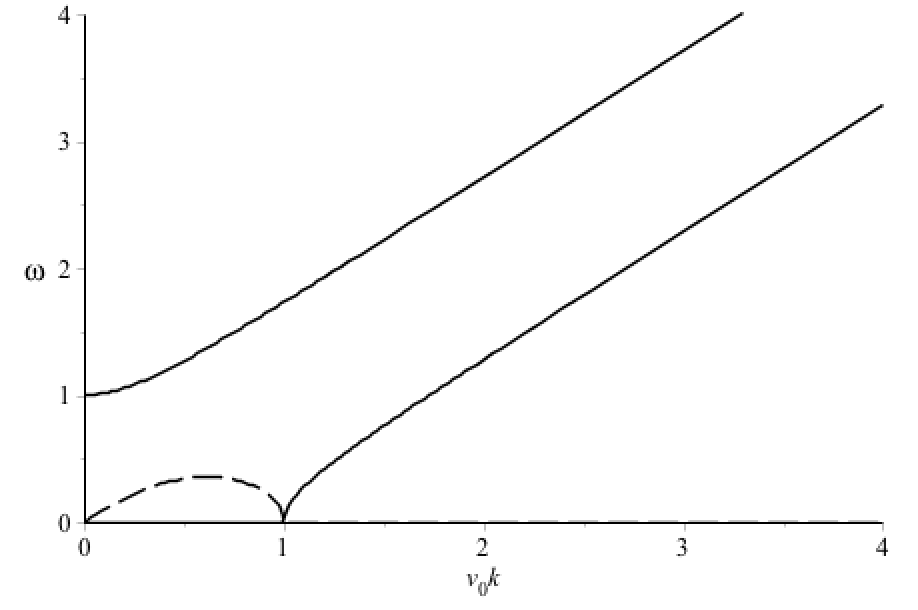
\includegraphics[height=10\baselineskip,width=0.3\textwidth]{Fig_2stream.png}
%\caption{Two stream instability}
%\label{Fig_2stream}
%\end{wrapfigure}

Note that here, $\omega_{p0}$ denotes the plasma frequency at the total (background) electron density $n_0$, while the beam (half-density) $n_0/2 = \langle n_e^{\pm}(t=0) \rangle$ was used in the lecture.


\subsection*{Exercise 6: Dispersion relation, characteristic frequencies and growth rate: Theory}

\begin{floatingfigure}[r]{0.4\linewidth}
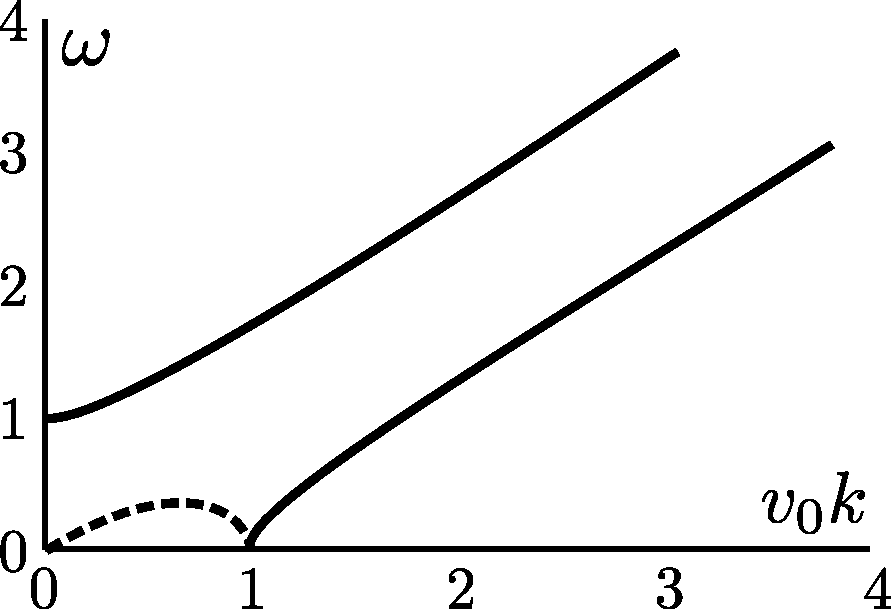
\includegraphics[width=0.4\linewidth]{Fig_2stream.pdf}
\caption{Two stream instability}
\label{Fig_2stream}
\end{floatingfigure}

{\bf (6.1)} For a given value of $v_0 k$, show that Eq.~\eqref{eq_disprel_2stream} is equivalent to the biquadratic equation on $\omega$:
\begin{eqnarray}\label{eq_biquad}
\omega^4 - (1+2 v_0^2 k^2)\,\omega^2 + v_0^2 k^2\,(v_0^2 k^2-1) = 0\,\,.
\end{eqnarray}
{\bf (6.2)} Solve Eq.~\eqref{eq_biquad} to obtain:
\begin{eqnarray}
\omega^2 = \frac{1}{2}\,\left[ (1+2 v_0^2 k^2) \pm \sqrt{1+8 v_0^2 k^2} \right]
\end{eqnarray}
Show that it admits imaginary solution for $v_0 k<1$. To what does this imaginary solution correspond to?\\
{\bf (6.3)} Plot, as a function of $v_0 k$ (e.g. in the range $0 - 5$),  the solution for $\omega$ (use dashed lines for the imaginary solution). [For the current exercise, you can directly use the plot given in Figure~\ref{Fig_2stream}]\\
{\bf (6.4)} Considering that the dispersion relation is obtained assuming all perturbed quantities vary as $\exp[i(\omega t - k\,x)]$, show that, for $v_0 k>1$, the energy in the electrostatic field varies as $A + B\,\cos(2\,\omega_a\,t) + C\,\cos(2\,\omega_b\,t) + D\,\cos[(\omega_a-\omega_b)\,t] + E\,\cos[(\omega_a+\omega_b)\,t]$, with $A$, $B$, $C$, $D$ and $E$ some numerical constants. What do $\omega_a$ and $\omega_b$ stand for?\\
{\bf (6.5)} Similarly, show that, for $v_0 k<1$, the energy in the electrostatic field goes as $A + B\,\cos(2\omega t) + C\,\cos(\omega t)\,\exp(\gamma t)+D\,\exp(2\gamma t)$. What do $\omega$ and $\gamma$ stand for? 

%\begin{figure}[h!]
%\centering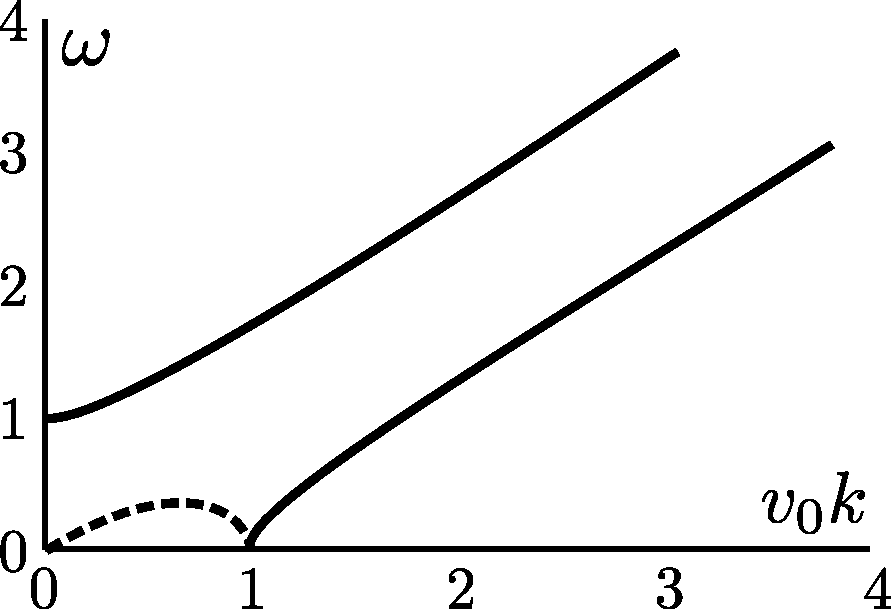
\includegraphics[width=0.5\textwidth]{Fig_2stream.pdf}
%\caption{Two stream instability}
%\label{Fig_2stream}
%\end{figure}


\subsection*{Numerical simulation of the 2-stream instability}

We will now perform numerical simulation using the PIC code SMILEI for different values of $v_0 k$.
As discussed above, we take $v_0=10^{-1}$ which ensures that relativistic effects can be neglected.
In addition, we use periodic boundary conditions, so that $k$ is uniquely defined by the simulation length using Eq.~\eqref{eq_k}.
The input file to start these simulation is given \texttt{TP\_proj2.py}.

\subsection*{Exercise 7: Simulation for $v_0 k > 1$}

\noindent{\bf (7.1)} Compute the values of $v_0 k$ corresponding to different values of $k$ using \\ \texttt{sim\_length} $= 0.62 - 0.60- 0.31 - 0.16$. Calculate the corresponding values of $\omega$ from Eq. (15).\\
\noindent{\bf (7.2)} Run the corresponding simulations.  For the phase-space diagnostics, in the input file \texttt{TP\_proj2.py}, take for the extremes values of the momentum in \texttt{DiagPhase} and \texttt{second[]}  $\mp 0.11$, respectively.For simulations with \texttt{sim\_length} $= 0.62$ and $0.60$, extract from the field energy temporal evolution the characteristic frequencies (try to estimate error bars for your measurements). Report them on the analytical predictions (from Exercise 6). Why does it become more difficult to extract the characteristic frequencies for \texttt{sim\_length} $= 0.31 - 0.16$ ?\\
\noindent{\bf (7.3)} Discuss the general behaviour of (i) the energy in the electrostatic field, and (ii) the behaviour in phase-space of the electron species. \\

\subsection*{Exercise 8: Simulation for $v_0 k < 1$}

\noindent{\bf (8.1)}  Compute the values of $v_0 k$ corresponding to \texttt{sim\_length} $= 0.69 - 1.03 - 1.68$. Calculate the corresponding values of $\omega$ and $\gamma$ from Eq. (15).\\Set the density perturbation $\delta n = 0.001$. \\
\noindent{\bf (8.2)} Run the corresponding simulations. For the phase-space diagnostics, in the input file \texttt{TP\_proj2.py},  take for the extremes values of the momentum in \texttt{DiagPhase} and \texttt{second[]}   to $\pm 0.4$, respectively. For each simulation (i.e. for different value of the parameter $v_0 k$), extract from the field energy temporal evolution the characteristic frequency and growth rate of the instability (it is convenient to consider the energy plot in log-scale. To do so, just click on the corresponding panel and letter `l'). Report them on the analytical predictions (from Exercise 6).\\
\noindent{\bf (8.3)} For each simulation, discuss the general behaviour of (i) the energy in the electrostatic field, and (ii) the behaviour in phase-space of the electron species. \\
\noindent{\bf (8.4)} For these simulations, using the temporal evolution of the electrostatic energy, discuss over what characteristic time the instability is in its linear phase.\\
\noindent{\bf (8.5)} Now, considering the phase-space distribution of the electron species, discuss what happens in the nonlinear phase of the instability.



%%%%%%%%%%%%%%%%
%  REFERENCES  %
%%%%%%%%%%%%%%%%



\begin{thebibliography}{2}

\bibitem{birdsall_langdon} C.~K.~Birdsall and A.~B.~Langdon, {\it Plasma physics via computer simulation}, McGraw-Hill, New York (1985).
\bibitem{taflove_2005} A.~Taflove and S.~C.~Hagness, {\it Computational Electrodynamics: The Finite-Difference Time-Domain Method}, 3rd~ed. Norwood, MA: Artech House (2005).
\bibitem{boris_1970} J.~P.~Boris, {\it Relativistic plasma simulations - Optimization of a hybrid code}, Proc. 4th Conf. Num. Sim. of Plasmas {\bf 3}, 1970.


\end{thebibliography}
\newpage
\section*{SMILEI namelists}
\lstinputlisting{TP_proj1.py}
\lstinputlisting{TP_proj2.py}


These notes are available at: \url{https://github.com/iltommi/TPUPMC}

The smilei code can be downloaded from \url{https://github.com/SmileiPIC/Smilei}

\end{document}


